% GeoMind TikZ 编译模板
% 编译方式：
%   xelatex tikz-template.tex
%
% 把 GeoMind「导出 → TikZ 代码」生成的
% \coordinate ... / \draw ... / \node ...
% 粘贴到下面的 tikzpicture 中即可。

\documentclass[border=10pt]{standalone}
\usepackage{ctex}
\usepackage{amsmath,amssymb}
\usepackage{tikz}
\usepackage{newunicodechar}

% GeoMind 标签中可能出现的 Unicode 下标
\newunicodechar{₀}{\ensuremath{_0}}
\newunicodechar{₁}{\ensuremath{_1}}
\newunicodechar{₂}{\ensuremath{_2}}
\newunicodechar{₃}{\ensuremath{_3}}
\newunicodechar{₄}{\ensuremath{_4}}
\newunicodechar{₅}{\ensuremath{_5}}
\newunicodechar{₆}{\ensuremath{_6}}
\newunicodechar{₇}{\ensuremath{_7}}
\newunicodechar{₈}{\ensuremath{_8}}
\newunicodechar{₉}{\ensuremath{_9}}
\newunicodechar{∠}{\ensuremath{\angle}}
\newunicodechar{°}{\ensuremath{^\circ}}
\newunicodechar{⊥}{\ensuremath{\perp}}
\newunicodechar{∥}{\ensuremath{\parallel}}

\begin{document}
% GeoMind · 竞赛几何工作台
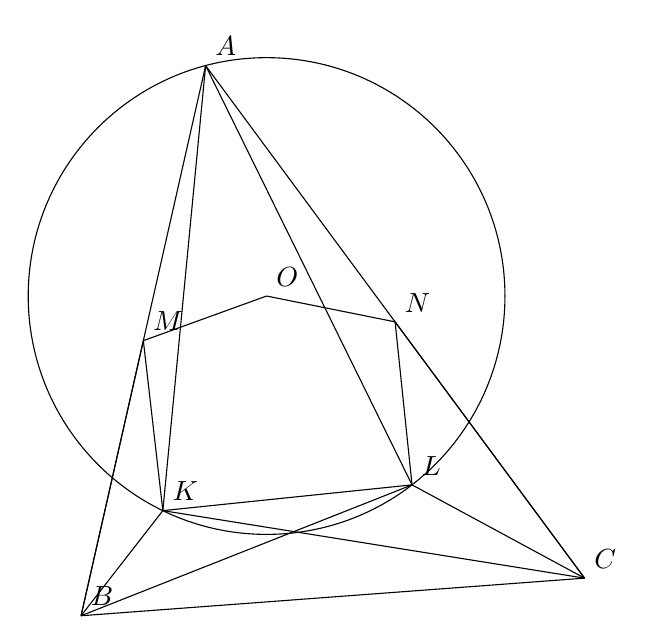
\begin{tikzpicture}[scale=1]
  \coordinate (A) at (-1.9904, 4.8553);
  \coordinate (B) at (-3.5723, -2.1318);
  \coordinate (C) at (2.8221, -1.6542);
  \coordinate (M) at (-2.7813, 1.3618);
  \coordinate (N) at (0.4159, 1.6005);
  \coordinate (K) at (-2.5337, -0.7967);
  \coordinate (L) at (0.631, -0.4696);
  \coordinate (O) at (-1.2162, 1.9287);
  \draw (A) -- (B);
  \draw (A) -- (C);
  \draw (B) -- (C);
  \draw (B) -- (M);
  \draw (C) -- (N);
  \draw (B) -- (K);
  \draw (B) -- (L);
  \draw (C) -- (K);
  \draw (C) -- (L);
  \draw (A) -- (K);
  \draw (A) -- (L);
  \draw (K) -- (L);
  \draw (O) -- (M);
  \draw (O) -- (N);
  \draw (L) -- (N);
  \draw (M) -- (K);
  \draw (-1.2162, 1.9287) circle (3.0272);
  \node[above right] at (A) {$A$};
  \node[above right] at (B) {$B$};
  \node[above right] at (C) {$C$};
  \node[above right] at (M) {$M$};
  \node[above right] at (N) {$N$};
  \node[above right] at (K) {$K$};
  \node[above right] at (L) {$L$};
  \node[above right] at (O) {$O$};
\end{tikzpicture}
\end{document}
